%!TEX root = ../document.tex
\setcounter{page}{1}
\pagenumbering{arabic}
\chapter{Introduction}
In this master thesis we will look at how students use a plant monitoring system called Monoplant to support their scientific inquiry when learning about photosynthesis. 

%Computer based technology are increasingly being used for educational purposes, both in school settings and student-initiated settings. As of 2009 every high school student in Norway should have a personal computer available for use (UDIR). The use of ICT is receiving increased attention as it is believed that it can enhance students learning and provide productive learning environments. One important point is that the usage of ICT is important in itself to prepare students for working with technology. However, making use of the opportunities these technologies give us, by applying digital content specifically designed for educational contexts, is in our opinion of equal importance. 

With the advent of Internet-connected embedded devices, we face an opportunity to distribute time consuming and tedious tasks to computers. By using digital sensors, one can initiate the collection of quantitative data from our surroundings and do other things while a computer handles monotonous tasks such as logging and storing the data. Say we want to conduct an experiment where we log the temperature throughout a day. Instead of walking over to the thermometer every 15 minutes to write down the temperature, a computer can read and store the temperature in a database. This technology has been used by meteorologists, scientists and commercial operators for a long time, but as the technology is becoming cheaper and more widespread, it is also becoming available for most people. %An important positive effect of this is of course that we can save a lot of time when gathering quantitative data, but we think a more interesting aspect is what can be done with this data. 

A increasingly popular usage is automation of tasks, as one can make the computer react to the data based on some preset thresholds regarding the values. There are for example automated watering systems that water plants based on readings of the soil moisture, or heating systems that turn on if the temperature is below a value. Automation can indeed take loads of work off our backs and thereby save us time. While there is truly a market for this, we think an even more interesting usage of such data exists and it consists of interpretation. The logged data can be accessed and presented in any way we want. This creates a great possibility for creating digital content from the real world and design it to be used in educational contexts.


\section{Motivations and background}
When we started working with ideas for this thesis, our goal was to do research on an actual product in a real world setting. As we chose to develop a system ourselves, a major part of the work on this thesis became to build and complete the system. In 2012 during a project in the course inf5261 - \emph{Development of mobile information systems} we developed a mixed reality game called Plantagotchi. The idea was to animate a digital version of a real plant, which was affected by how the real plant was treated. In this project the user group was children at the age of 8-12 and the system was planned to be used as a school contest where classes competed in getting the happiest plant. The educational outcome being pupil motivation for learning about growth conditions for plants, so that they could win the game. The prototype developed in this course became the foundation of the system in this thesis referred to as Monoplant.

\begin{figure}
\centering
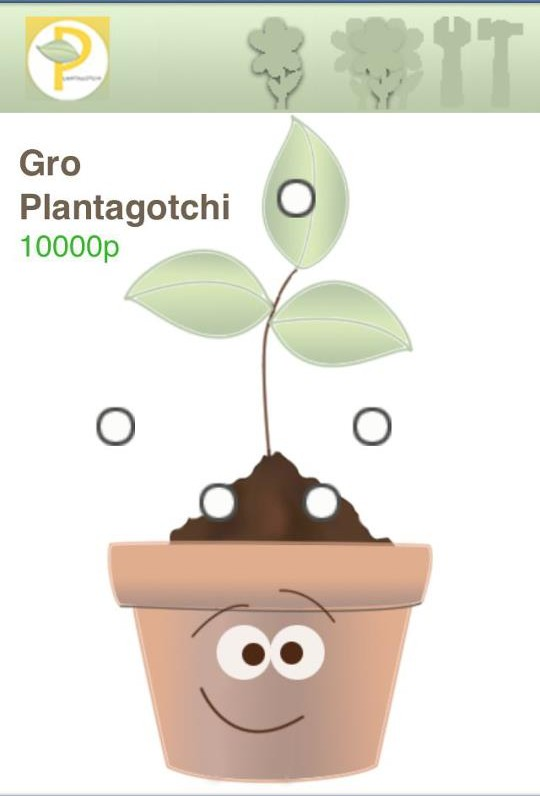
\includegraphics[width=0.5\textwidth]{img/introduction/plantagotchi.jpg}
\caption{Screenshot of Plantagotchi prototype}
\label{fig:scrshotplantagotchi}
\end{figure}

During the spring of 2013 we both took the course inf5790 \emph{Technology enhanced learning} where we were introduced to the field of Computer Supported Collaborative Learning (CSCL). As we brought with us an idea of an application that pupils could use to collaboratively learn about a scientific domain, CSCL became the field where we could adapt theoretical perspectives and concepts, which set words to and explained our personal ideas and experiences. 

The starting point of this thesis was to do research on an actual working system, in an authentic environment. We therefore brought with us the ground idea from Plantagotchi and spent a lot of time improving it and developing a new working prototype. In October 2013 we got in touch with a school, and had a fully working plant monitoring system that we could test with real users in their natural setting. The focus in this thesis is therefore directed to this design experiment performed in a high school biology class. We will also provide some background information about the decisions made while developing our educational system, Monoplant. 


\section{Monoplant}
Plants live a slow life, they grow slowly and move slowly. Human beings do not have the patience to watch a plant grow, but we are able to see that it has grown or bloomed. However, humans do have the ability to use tools in order to make sense of the world, and we have created such a tool: Monoplant, which can help us see how plants evolve over time.

Monoplant is a monitoring system for plants, or rather humans who want to monitor their plants. It continuously gathers data about a plant's environment and makes the data available to the users via the Internet. One functionality is thereby to remotely monitor a plant and get instant data about temperature, humidity, light, soil moisture and even a picture of the plant. 

However, one of the main reasons for designing Monoplant, was that we wanted to see how plants develop over time, or in biological terms their ontogenetic development. Hence we tried to combine readings over time to see if we were able to observe if some of the variables affected the plant physically. The first step became to merge the images taken into a time-lapse video. This made it possible to see a plant's physical development throughout a day in a matter of seconds. In order to link this with the variables from the environment, we had to connect each image in the video to its corresponding data reading. This is done by presenting a graph together with the time-lapse video and marking the point in the graph which corresponds to the current image in the video (see figure~\ref{fig:scrshotgraphlapse}). Thus we are connecting \emph{visible} changes of the plant (i.e., the video) to \emph{invisible} changes in the environment (e.g., soil moisture and humidity levels).


\begin{figure}
	\centering
	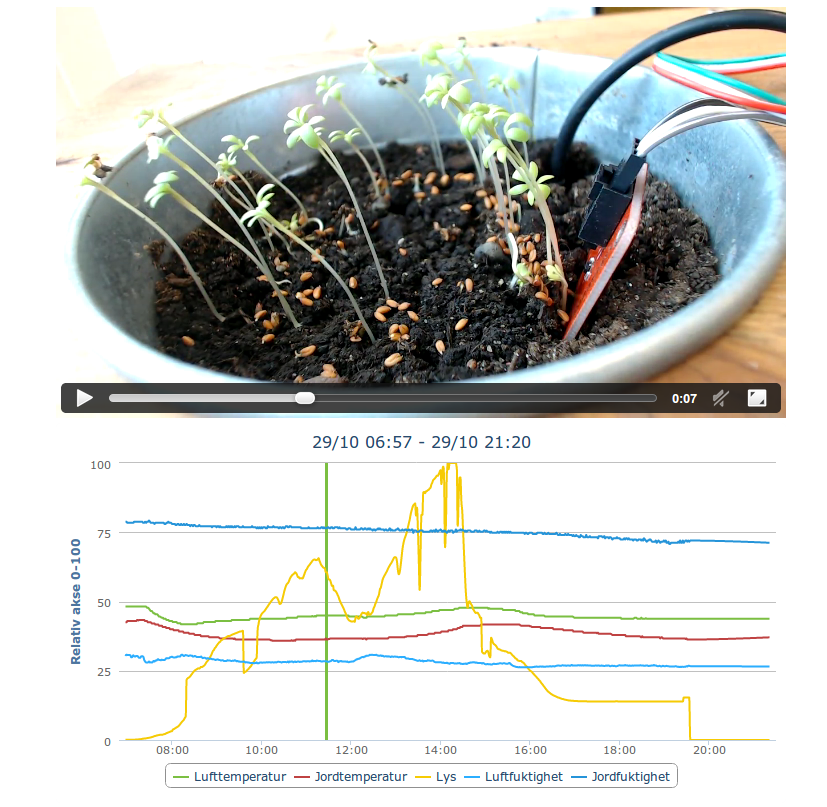
\includegraphics[width=\textwidth]{img/introduction/graphlapse.png}
	\caption{Screenshot of timelapse and graph}
	\label{fig:scrshotgraphlapse}
\end{figure}

%Maybe write something about how this is generic, but that in this thesis we have chosen to focus on how it can be used in learning.

\section{Research questions}
%place our focus in the CSCL field
As mentioned, the overall theme of this thesis is how students can use Monoplant in their scientific inquiry when learning about photosynthesis in a biology class. This will be investigated through an analysis of a study performed in the autumn of 2013. In order to address this broad theme we will try to answer four research questions.


\begin{noindlist}
\item \emph{"What characterizes the students’ inquiry in interaction with Monoplant?"}\\
This will naturally adress the characteristics of the students' actions and interactions during their work with Monoplant. The first question will also be elaborated through the next three questions.
\item \emph{"How does Monoplant, by presenting photosynthesis differently from how it is rendered in the text book, support the inquiry process?"}\\
This question is indicating that there is a difference between the representation of photosynthesis in the school textbook and in Monoplant. To answer this we will address these differences, and discuss what implications they have in the students' inquiry process.
\item \emph{"In what way is scaffolding operationalized in the environment?"}\\
For this question to make sense, we need to introduce the theoretical concept of \emph{scaffolding} and put it in a broader context of instructional theory. This will be elaborated later in the thesis, but for now we can call it training wheels. We will look at how the teacher and Monoplant help the students in their inquiry process.
\item \emph{"How does the institutional setting frame the students' inquiry process?"}.\\
As the study took place in a school setting, we wanted to look at how the social practices within school affected the inquiry process.
\end{noindlist}

Although all of our research questions sets a focus towards describing characteristics of student interaction in our design experiment, we will also try to be prescriptive in terms of further research to be done and improvements in the design of Monoplant.

\section{Thesis outline}
%scientific backgroud 
%technical background
%theory
%empirical & method
%data and analysis
%discussion
%concluding remarks
We will now present an outline for this thesis, providing an overview of the contents as well as the structure. 

\subsubsection*{Chapter 1 - Introduction}
The introduction presents our personal and professional motivations for writing this thesis, a brief introductions to Monoplant followed by the research questions, and lastly this "readers guide".

\subsubsection*{Chapter 2 - Scientific background}
This chapter is an introduction to photosynthesis and thereby the scientific language within the domain. The introduction represents what the students in our case are supposed to learn in \emph{Biology 2}. It is provided as a tool to understand what we mean later in the thesis when using domain specific terms such as \emph{"light dependent reaction"}, \emph{"excited"} or \emph{"chlorophyll molecules"}.

\subsubsection*{Chapter 3 - Technical architecture and programming}
%The application is divided into three logical units: data collection, data processing and database, and user interface. In the following sections these units will be explained further. 
A major part of the work done for this thesis to become a reality was to design and build Monoplant. In this chapter we will describe Monoplant's architecture and address some of the technical concerns we met during the development process. We will introduce \emph{Raspberry Pi}, \emph{Arduino}, \emph{Ruby on Rails}, \emph{REST} and other frameworks and tools used to build Monoplant.

\subsubsection*{Chapter 4 - Theoretical perspective and concepts for analysis}
%In this chapter we will lay forth the theoretical perspective and theoretical concepts we will apply in this thesis. First we will introduce the \emph{sociocultural perspective} and highlight some key points including \emph{institutional practices}, \emph{zone of proximal development} and \emph{scaffolding}. Further we will look at \emph{multiple external representations} and lastly the concept and method of \emph{Inquiry learning}.

%In this chapter we will present the sociocultural perspective, which will be used throughout this thesis. We will also introduce the theoretical concepts: \emph{spontanous and scientific concepts}, \emph{zone of proximal developement (ZPD)}, \emph{scaffolding}, \emph{multiple external representations (MER)}, \emph{institutional settings}, \emph{inquiry learning} and \emph{misconceptions}. We will make an account for our interpretation of these concepts as we will use them later in the thesis in order to answer our research questions. 

In this chapter we will present the sociocultural perspective, along with the theoretical concepts: \emph{spontanous and scientific concepts}, \emph{zone of proximal developement (ZPD)}, \emph{scaffolding}, \emph{multiple external representations (MER)}, \emph{institutional settings}, \emph{inquiry learning} and \emph{misconceptions}. Focus will lie on our interpretation as we will use them later in the thesis in order to answer our research questions. 

\subsubsection*{Chapter 5 - Empirical setting and method}
%In this chapter, we will present the empirical setting and methods used in this thesis. First we will describe the empirical setting in which the data collection took place. Then we will proceed to present the methods for gathering data with a description of the technicalities of the data. Lastly, we will describe the procedures for selection and analysis of data.

Throughout October 2013 we gathered data for this thesis. In this chapter we will introduce \emph{design based research} together with the \emph{systemic} and \emph{dialogic} approach. We describe the empirical setting in which the data gathering took place, along with the methods used for collecting the data and how we used those methods. Then we will explain how we approached, selected and made sense of the data once the data collection was done. Lastly, the quality of our research will be addressed. 

\subsubsection*{Chapter 6 - Data and analysis}
%In this chapter we will present the findings from our case study with a focus on themes relevant to our research questions. Each of the themes contain at least one excerpt with a context description, excerpt from the transcript, and an analysis of the unfolding events.
Here we will present the main findings from our study. The chapter contains ten data extracts, which are presented one by one. First by a context description, then a data transcript and finally a clarification and analysis of what happened. 

\subsubsection*{Chapter 7 - Discussion}
%In this chapter we discuss our research questions by contextualizing our findings according to the theoretical concepts introduced earlier. As an overall theme we look at the inquiry process of the students in interaction with Monoplant. This will be showed through 4 sections, the first being about the inquiry process itself. Next we will discuss how multiple external representations support the inquiry process of the students. Then how scaffolding is instantiated in the environment, and finally how the institutional setting frame the students' inquiry process.
In this chapter we will discuss our research questions by applying the theoretical concepts introduced in chapter 4 to our findings in chapter 7. Our first research question \emph{"What characterizes the students’ inquiry in interaction with Monoplant?"} will be the overall theme of this chapter, but all four of the questions will be addressed.

\subsubsection*{Chapter 8 - Concluding remarks}
Our concluding remarks will provide the reader with an overview of how we approached this thesis and a review of our main findings according to the research questions. Lastly we will present shortcomings and suggestions for further work.